\documentclass{book}
\usepackage{graphicx}
\usepackage[english]{babel}
\usepackage{amsthm}
\usepackage{amssymb}
\usepackage{amsfonts}
\usepackage{cancel}
\usepackage{mathrsfs}
\usepackage{physics}
\usepackage{tikz}
\usepackage[a4paper, margin=1in]{geometry}
\geometry{a4paper, margin=1in}
\usepackage{xcolor}
\usetikzlibrary{arrows.meta}
\usetikzlibrary{angles,quotes}
\graphicspath{ {./images/} }
\usepackage{svg}
\usepackage{subcaption}
\usepackage{bm}
\usepackage{empheq}
\usetikzlibrary{decorations.text}
\usepackage[most]{tcolorbox}
\usepackage{tensor}
%3D
\usepackage{mathtools}
\usepackage{booktabs}
\usepackage{array}
\newcolumntype{C}{>{$}c<{$}}
\usepackage{tikz-3dplot}
\usepackage{appendix}
\usepackage{pgfplots}
\usetikzlibrary{shapes.geometric}
\usetikzlibrary{calc,patterns,angles,quotes}
%Tikz Library
\usetikzlibrary{angles, quotes, intersections}
\usepackage[bb=dsserif]{mathalpha}
\usetikzlibrary{decorations.pathmorphing}

\tikzset{snake it/.style={decorate, decoration=snake}}
\usepackage{mdframed}

\usepackage{etoolbox} % ifthen
\usepackage[outline]{contour} % glow around text
\usetikzlibrary{calc} % for adding up coordinates
\usetikzlibrary{decorations.markings,decorations.pathmorphing}
\usetikzlibrary{angles,quotes} % for pic (angle labels)
\usetikzlibrary{arrows.meta} % for arrow size
\usepackage{xfp} % higher precision (16 digits?)

\renewcommand{\cleardoublepage}{\clearpage}

\title{Mathematics of Waves and Fields}
\author{Dominik Szablonski}
\newtheorem{law}{Law}
\newtheorem{klaw}{Law}
\newtheorem*{definition}{Definition}
\newtheorem*{theorem}{Theorem}

\newenvironment{aside}
{\begin{mdframed}[style=0,%
		leftline=false,rightline=false,leftmargin=2em,rightmargin=2em,%
		innerleftmargin=0pt,innerrightmargin=0pt,linewidth=0.75pt,%
		skipabove=7pt,skipbelow=7pt]\small}
	{\end{mdframed}}

\pgfplotsset{compat=1.18}
\begin{document}
\maketitle

\tableofcontents

\chapter{Partial Differential Equations}
\section{Separation of Variables}
Suppose we have a PDE whose solution is in the form, $u(r_1,r_2,\ldots,r_n)$ where there are $n$ co-ordinates $r_i$, then we can solve the PDE by separation of variables by assuming a solution of the form,
\begin{equation}
	u(r_1,r_2,\ldots,r_n) = R_1(r_1)R_2(r_2)\cdots R_n(r_n).
\end{equation}
This will turn a compatible PDE into an ODE.
\subsection{Specific solutions}
We are often most interested in the specific solutions to a wave equation. In order to get a specific solution, constraints/boundary conditions must be provided. The general method is as follows,
\begin{enumerate}
	\item Use separation of variables;
	\item Build superpositions of solutions;
	\item Apply boundary conditions and find appropriate constants.
\end{enumerate}
\section{Series Solutions}
The general steps to solving an ODE using this method are,
\begin{enumerate}
	\item Assume a series solution of the form,
	\begin{equation}
		y = \sum_{n=0}^{\infty}a_kx^k
	\end{equation}
	\item Obtain the recurrence relation.
\end{enumerate}
\chapter{Fourier Series}
Given a periodic function $f(x)$ with period $2L$ in the range $-L \leq x \leq L$, the Fourier expansion is given by,
\begin{equation}
	\boxed{
	f(x) = \frac{a_0}{2} + \sum_{n=1}^{\infty}\left(a_n \cos \frac{n\pi x}{L} + b_n \sin\frac{n\pi x}{L}\right)
	}
\end{equation}
for,
\begin{align}
	\boxed{a_n = \frac{1}{L}\int_{-L}^{L}f(x)\cos\frac{n\pi x}{L}\dd{x}} && \boxed{b_n = \frac{1}{L}\int_{-L}^{L} f(x)\sin\frac{n\pi x}{L} \dd{x}}
\end{align}
In order to expand a function it must meet \textit{Dirichlet's Conditions}, so the function must,
\begin{enumerate}
	\item be single valued,
	\item have a finite number of discontinuities,
	\item $\int_{-L}^L|f(x)|\dd{x}$ must be finite.
\end{enumerate}
We say that $\sin \frac{n\pi x}{L}$ and $\cos\frac{n \pi x}{L}$ form a \textit{complete, orthogonal basis}. And furthermore, the Fourier series allows \textit{an expansion of a function on a set of orthogonal basis functions}.
\section{Exponential Fourier Series}
We can further write the Fourier expansion in terms of complex exponentials,
\begin{equation}
	\boxed{f(x) = \sum_{n = -\infty}^{\infty} c_n \exp\left(i \frac{n\pi x}{L}\right)}
\end{equation}
for,
\begin{equation}
	\boxed{c_n = \frac{1}{2L}\int_{-L}^{L}f(x)\exp\left(-i\frac{n\pi x}{L}\right)\dd{x}}
\end{equation}
From our complex definition of the Fourier series, we can say that 2 complex functions $u(z)$ and $v(z)$ are orthogonal on the interval $a \leq z \leq b$ if,
\begin{equation}
	\int_a^b u(z)v(z) = 0.
\end{equation}
\chapter{Fourier Transform}
If we wish to analyse non-periodic functions, we can take the limit of our range, $\lim_{L\to\infty}(-L,L)$. Let us write,
\begin{align}
	k_n = \frac{n\pi}{L} && \Delta k = \frac{\pi}{L}
\end{align}
so,
\begin{align}
	 \\
	c_n & = \frac{1}{2L}\int_{-L}^{L}f(x)\exp\left(-ik_nx\right)\dd{x}.
\end{align}
Let us write $F(k) = 2Lac_n$,
\begin{align}
	F(k_n) = a\int_{-L}^{L}f(x)\exp\left(-ik_nx\right)\dd{x} \\
	\implies f(x) &= \frac{1}{2\pi a}\sum_{n = -\infty}^{\infty} F(k_n)\exp\left(i k_nx\right)\Delta k.
\end{align}
In the limit of $L \to \infty$, we obtain,
\begin{align}
	\boxed{F(k) = a\int_{-\infty}^{\infty}f(x)\exp(-ikx)\dd{x}} && \text{Fourier transform of $f(x)$.}\\
	\boxed{f(x) = \frac{1}{2\pi a}\int_{-\infty}^{\infty}F(k)\exp(ikx)\dd{k}} && \text{Inverse Fourier transform of $F(k)$.}
\end{align}
We define constant,
\begin{equation}
	a = \begin{dcases}
		\text{unity} & \text{Physics} \\
		\frac{1}{\sqrt{2\pi}} & \text{Maths}
	\end{dcases}.
\end{equation}
\section{Manipulation of the Fourier transform}
Most generally,
\begin{equation}
	\boxed{\mathscr{F}\left\{f(ax - b)\right\} = e^{-ikb}\frac{1}{a}F\left(\frac{k}{a}\right)}.
\end{equation}

\section{Dirac-Delta Function}
Dirac's original approximation of the $\delta$ function used a function $\Pi(x)$ which was defined,
\begin{equation}
	\Pi(x) = \begin{dcases}
		1 & -\frac{1}{2} \leq x \leq \frac{1}{2} \\
		0 & \text{Elsewhere}
	\end{dcases}.
\end{equation}
Using this definition we can write,
\begin{equation}
	\delta(x) = \lim_{k \to \infty} \left\{k\Pi(kx)\right\}.
\end{equation}
It can also be defined using $\mathrm{sinc}$,
\begin{equation}
	\delta(x) = \lim_{k \to \infty}\left\{\frac{k}{\pi}\frac{\sin{kx}}{kx}\right\}.
\end{equation}
However, the most commonly used, and most applicable form is,
\begin{equation}
	\boxed{\delta(x) = \frac{1}{2\pi}\int_{-\infty}^{\infty}e^{ikx}\dd{x} = \frac{1}{2\pi}\int_{-\infty}^{\infty}e^{-ikx}\dd{x}}
\end{equation}
We note 4 important properties of the Dirac-Delta,
\begin{enumerate}
	\item $\displaystyle \lim_{x \to 0}\delta(x) = \infty$ 
	\item $\displaystyle \int_{-\infty}^{\infty}\delta(x)\dd{x} = 1$
	\item $\displaystyle \delta(ax + b) = \dfrac{1}{|a|}\delta\left(x + \dfrac{a}{b}\right)$
	\item $\delta(x) = \delta(-x)$ i.e., Dirac-Delta is even.
\end{enumerate}
\subsection{Fourier Transform of the Dirac Delta}
The Fourier transform of a constant is the Dirac-Delta, i.e.,
\begin{align}
	\mathscr{F}\left\{1\right\} = \int_{-\infty}^{\infty}e^{ikx}\dd{x} = 2\pi\delta(x),
\end{align}
and similarly for the inverse Fourier Transform,
\begin{equation}
	\mathscr{F}^{-1}\left\{1\right\} = \frac{1}{2\pi}\int_{-\infty}^{\infty}e^{ikx}\dd{x} = \delta(x).
\end{equation}
Taking the Fourier transform of the Dirac-Delta,
\begin{equation}
	\mathscr{F}\left\{\delta(x)\right\} = \int_{-\infty}^{\infty}\delta(x)e^{-ikx}\dd{x} = 1
\end{equation}
and thus clearly,
\begin{equation}
	\mathscr{F}\left\{\delta(x - x_0)\right\} = \int_{-\infty}^{\infty}\delta(x - x_0)e^{-ikx}\dd{x} = e^{-ikx_0}.
\end{equation}

\section{Parseval's Theorem}
\begin{theorem}
\begin{equation}
	\boxed{\int_{-\infty}^{\infty} \left|f(x)\right|^2\dd{x} = a\int_{-\infty}^{\infty}\left|F(k)\right|^2\dd{k}}
\end{equation}
where $a=1$ for mathematical symmetry, and $a= \frac{1}{2\pi}$ for physical symmetry.
\begin{proof}
	\begin{equation}
		\begin{split}
		\int_{-\infty}^{\infty}\left|f(x)\right|^2\dd{x} &= \frac{1}{2\pi}\int_{-\infty}^{\infty}\int_{-\infty}^{\infty}F(k)e^{ikx}\dd{k}\int_{-\infty}^{\infty}F^*(k)e^{ik'x}\dd{k'}\dd{x}\\
		& = \int_{-\infty}^{\infty}F(k)\dd{k}\int_{-\infty}^{\infty}F^*(k')\dd{k'}\underbrace{\frac{1}{2\pi}\int_{-\infty}^{\infty}e^{i(k-k')x}\dd{x}}_{\delta(k-k')} \\
		& = \int_{-\infty}^{\infty}\left|F(k)\right|^2 \dd{k}
		\end{split}
	\end{equation}
\end{proof}
\end{theorem}
\section{Convolution}
We define the convolution $h(x)$ of two functions $f(x)$ and $g(x)$ as,
\begin{equation}
	\begin{split}
		h(x) = f(x) * g(x) & = \int_{-\infty}^{\infty}f(x - x')g(x')\dd{x'} \\
		& = \int_{-\infty}^{\infty}f(x')g(x - x')\dd{x'}.
	\end{split}
\end{equation}
If we define the Fourier transforms of $f(x)$ and $g(x)$,
\begin{align}
	F(k) = \mathscr{F}\left\{f(x)\right\} && G(k) = \mathscr{F}\left\{g(x)\right\}
\end{align}
then the Fourier transform of the convolution is given by,
\begin{equation}
	\mathscr{F}\left\{h(x)\right\} = \mathscr{F}\left\{f(x) * g(x)\right\} = F(k)G(k).
\end{equation}
\begin{proof}
	Let us define $\zeta = x - x'$, then,
	\begin{equation}
		\begin{split}
			H(k) & = \int_{-\infty}^{\infty}\int_{-\infty}^{\infty}\dd{x}\dd{x'}f(\zeta)g(x')e^{-kx} \\
			& = \int_{-\infty}^{\infty}\int_{-\infty}^{\infty} \dd{x'}\dd{\zeta}f(\zeta)g(x')e^{-ik(\zeta+x')} \\
			& = \int_{-\infty}^{\infty}g(x')e^{ikx'}\dd{x'}\int_{-\infty}^{\infty}f(\zeta)e^{ik\zeta}\dd{\zeta}
		\end{split}
	\end{equation}
	which clearly corresponds to the product of the two transforms.
\end{proof}
\section{Wave Packets}
In 1 dimension, a forward travelling wave is defined by,
\begin{equation}
	\phi(x,t) = e^{-i\left(kx - \omega t\right)}
\end{equation}
which satisfies the 1 dimensional wave equation,
\begin{equation}
	\pdv[2]{\phi}{x} = \frac{1}{c^2}\pdv[2]{\phi}{t}.
\end{equation}
By substituting in the travelling wave, we find,
\begin{align}
	k^2 = \frac{1}{c^2}\omega^2 \implies \omega = ck. 
\end{align}
A plane wave $\phi(\vb{x},t) = e^{i(\vb{k}\cdot\vb{x} - \omega t)}$ satisfies the 3 dimensional wave equation,
\begin{equation}
	\grad^2\phi = \frac{1}{c^2}\pdv{\phi}{t}.
\end{equation}
Where we have,
\begin{equation}
	\omega = c|k|
\end{equation}
for a plane travelling along $k$.
\\\\
Returning to the 1 dimensional wave, we can sum these travelling waves along the $+x$ direction,
\begin{equation}
	\phi(x,t) = \frac{1}{\sqrt{2\pi}}\int_{-\infty}^{\infty}G(k)e^{ik(x-ct)}\dd{k}
\end{equation}
where $G(k)$ is the Fourier transform os $\phi(x,0)$. This wave satisfies the wave equation as all components of the wave travel at the same velocity $c$. We are also able to use the wave equation to describe waves in \textit{non-dispersive media}, i.e., those where the velocity of the waves depends on wavelength,
\begin{equation}
	v_p(k) = \frac{\omega(k)}{k}.
\end{equation}
The most general wave can be written as,
\begin{equation}
	\boxed{\phi(x,t) = \frac{1}{\sqrt{2\pi}}\int_{-\infty}^{\infty}G(k)e^{i(kx - \omega(t)t)}\dd{k}}.
\end{equation}
\subsection{Dispersion}
A dispersive wave packet will have the following properties,
\begin{itemize}
	\item The envelope wave of the wave packet will move with group velocity,
	\begin{equation}
		\boxed{v_g = \dv{\omega}{k} = v_p + k\dv{v_p}{k}}.
	\end{equation}
	\item The dispersive effects of the wave are a second order effect. i.e., we must expand any approximations to the second order. We will always assume $\omega \equiv \omega(k)$.
\end{itemize}
\chapter{Special Functions}
\section{Taylor Expansion}
The Taylor expansion about $x_0$ is,
\begin{equation}
	\begin{split}
		f(x) & = f(x_0) + (x-x_0)f'(x) + \frac{(x-x_0)^2}{2!} + \cdots \\
		& = \sum_{n=0}^{\infty}f^{(n)}(x_0)\frac{(x-x_0)^n}{n!}
	\end{split}
\end{equation}
Let us then redefine this as a simple series,
\begin{equation}
	f(x) = \sum_{n=0}^{\infty}u_n
\end{equation}
we can then define the convergence criteria,
\begin{equation}
	\lim_{n\to\infty}|r_n| = \lim_{n\to\infty}\left|\frac{u_{n+1}}{u_n}\right| < 1.
\end{equation}
\section{Hermit's Equation}
\begin{equation}
	\dv[2]{y}{x} - 2x\dv{y}{x} + 2ny = 0, \forall y, n \in \mathbb{Z}
\end{equation}
We can obtain solutions to Hermit's equation by assuming a series solution,
\begin{equation}
	y = \sum_{k=0}^{\infty}x^k.
\end{equation}
Substituting this into Hermit's equation,
\begin{equation}
	\sum_{k=0}^{\infty}k(k-1)a_kx^{k-2} - 2x\sum_{k=0}^{\infty}ka_kx^{k-1} + 2n\sum_{k=0}^{\infty}a_kx^k = 0
\end{equation}
Let us shift $k$ such that, $k \to k + 2$,
\begin{equation}
	\begin{split}
		\sum_{k=0}^{\infty}(k+2)(k+1)a_{k+1}x^k - 2\sum_{k=0}^{\infty}ka_kx^k + 2n\sum_{k=0}^{\infty}a_kx^k & = 0 \\
		\sum_{k=0}^{\infty}\left\{(k+2)(k+1)a_{k+2} - (2k-2n)a_{k}\right\}x^k = 0
	\end{split}
\end{equation}
from which we obtain the recurrence relation,
\begin{equation}
	a_{k+2} = \frac{2(k-n)}{(k+2)(k+1)}a_n.
\end{equation}
Using this recurrence relation, we are able to form a solution for $y$, starting at $k=0$ and $k=1$ to obtain the even and odd solutions respectively,
\begin{equation}
	\begin{split}
		y = & a_0\left[1 - \frac{2n}{2!}x^2 - \frac{2n(4-2n)}{4!}x^4 + \cdots\right] + \\
		& a_1\left[x + \frac{(2-2n)}{3!}x^3 + \frac{(2-2n)(6-2n)}{5!}x^5 + \cdots\right]. \label{eq:hermit solution} 
	\end{split}
\end{equation}
Let us note that at $k=n$ the series will terminate.
\\\\
Given the solution to Hermit's equation, by considering different values of $n$, we are able to obtain \textit{Hermit's Polynomials} which are discussed in the section below.
\subsection{Hermit's Polynomials}
We denote Hermit's polynomials by $y \equiv H_n(x)$. By simply looking at eq. \eqref{eq:hermit solution}, we see that the first three even Hermit polynomials are,
\begin{align}
	H_0(x) = 1 && H_2(x) = 1 - 2x^2 && H_4(x) = 1 - 4x^2 + \frac{4}{3}x^4,
\end{align}
and the first 3 odd ones are,
\begin{align}
	H_1(x) = x && H_3(x) = x - \frac{2}{3}x^3 && H_5(x) = x - \frac{4}{3}x^3 + \frac{4}{5}x^5
\end{align}
In physics, we often normalise the Hermit polynomials such that the highest order term is positive and has a coefficient $2^n$.
\subsubsection{Orthogonality of Hermit Polynomials}
Hermit Polynomials satisfy the orthogonality relation,
\begin{equation}
	\int_{-\infty}^{\infty}H_n(x)H_m(x)e^{x^2}\dd{x} = \sqrt{\pi}n!2^m \delta_{nm}.
\end{equation}
This means that Hermit's polynomials can be used as a basis for series expansion of a function. We can further define a normalised Hermit function,
\begin{equation}
	\psi_m(x) = \left(\frac{1}{\sqrt{\pi}m!2^m}\right)^{1/2}H_me^{\frac{x^2}{2}}
\end{equation}
which satisfies,
\begin{equation}
	\int_{-\infty}^{\infty}\psi_m(x)\psi_n(x)\dd{x} = \delta_{mn}
\end{equation}
\section{Legendre's Equation}
\begin{equation}
	\boxed{(1-x^2)\dv[2]{y}{x} - 2x\dv{y}{x} + \ell(\ell + 1)y = 0 \hspace{10pt} l\geq 0, l \in \mathbb{Z}} \label{eq:legendre}
\end{equation}
We solve Legendre's equation by series expansion, from which we obtain,
\begin{equation}
	(1-x^2)\sum_{n=2} n(n-1)a_nx^{n-2} -2x\sum_{n=1}na_nx^{n-1} \ell(\ell + 1)\sum_{n=0}a_nx^n.
\end{equation}
Let us shift the sums so we only have terms in powers of $n$,
\begin{equation}
	\sum_{n=0} \left\{(n+2)(n+1)a_{n+2} - n(n-1)a_n - 2na_nx^n - 2na_nx^n + \ell(\ell + 1)a_n\right\}x^n = 0.
\end{equation}
From which we can easily obtain a general recurrence relation,
\begin{equation}
	\boxed{a_{n+2} = \frac{n(n+1) - \ell(\ell +1)}{(n+2)(n+1)}a_n}
\end{equation}
thus the solution for Legendre's equation has even and odd parts given below,
\begin{equation}
	\begin{split}
	y = & a_0\left[(1 - \ell(\ell +1))\frac{x^2}{2!} + (\ell - 2)(\ell(\ell +1)(\ell +3))\frac{x^4}{4!} + \cdots \right] \hspace{27pt} \text{Even} \\
	& + a_1\left[x - (\ell - 1)(\ell +2)\frac{x^3}{3!} + (\ell -3)(\ell -1)(\ell +2)\frac{x^5}{5!} + \cdots\right] \hspace{10pt} \text{Odd}
\end{split}
\end{equation}
which we can clearly see terminates at $\ell = n$, which allows the series to converge. 
\subsection{Legendre Polynomials}
The steps to finding Legendre polynomials $P_n(x)$ are as follows,
\begin{itemize}
	\item Decide whether the polynomial is odd or even, and choose which part of $y$ you will use.
	\item Find the coefficients of the polynomial $y(x)$ in terms of $a_0$ for even polynomials and $a_1$ for odd polynomials.
	\item Set $y(0) = 1$ to find a value for $a_1$ or $a_0$.
	\item Evaluate the final polynomial.
\end{itemize}
\subsubsection{Orthogonality of Legendre Polynomials}
Legendre polynomials are orthogonal over the interval $|x| \leq 1$, i.e.,
\begin{equation}
	\int_{-1}^{1} P_l(x) P_{m}(x) \dd{x} = 0 \hspace{10pt} m \neq l.
\end{equation}
Let us recall eq. \eqref{eq:legendre}, and rewrite,
\begin{align}
	\dv{x}\left[(1-x^2)\pdv{P_l}{x}\right]& = - l(l+1)P_l(x) \label{eq:fdh}\\
	\dv{x}\left[(1-x^2)\pdv{P_m}{x}\right]& = - m(m + 1)P_m(x). \label{eq:fdh2}
\end{align}
Multiply eq. \eqref{eq:fdh} by $P_m$, and eq. \eqref{eq:fdh2} by $P_l$, and take them away from each other. We have,
\begin{equation}
	\begin{split}
		\text{LHS} = & \int_{-1}^{1}\dv{x}\left[(1-x^2)\pdv{P_l}{x}\right]P_m\dd{x} \\
		& -\int_{-1}^{1}\dv{x}\left[(1-x^2)\pdv{P_m}{x}\right]P_l\dd{x}
	\end{split}\label{eq:4.23}
\end{equation}
Evaluating eq. \eqref{eq:4.23} by parts, we have,
	\begin{align}
		u = P_m && \dv{v}{x} = \dv{x}\left[(1-x^2)\pdv{P_l}{x}\right] \\
		\dv{u}{x} = \pdv{P_m}{x} && v = (1-x^2)\pdv{P_l}{x}
	\end{align}
and similarly for the latter half of the equation. we can then write,
\begin{equation}
	\begin{split}
		\text{LHS} = & \underbrace{\left[(1-x^2)\dv{P_l}{x}P_m\right]_{-1}^{1}}_0 - \int_{-1}^{1} (1-x^2) \dv{P_m}{x}  \dv{P_l}{x}\dd{x} \\
		& - \underbrace{\left[(1-x^2)\dv{P_m}{x}P_l\right]_{-1}^{1}}_0 - \int_{-1}^{1}(1-x^2)\dv{P_l}{x} \dv{P_m}{x}\dd{x} \\
		= & 0
	\end{split}
\end{equation}
We then have that, for $n\neq m$, the LHS is,
\begin{equation}
	\left[m(m+1)-l(l+1)\right]P_{l}(x)P_m(x) = 0
\end{equation}
Furthermore, we can show,
\begin{equation}
	\boxed{\int_{-1}^1 P_l(x)P_m(x) \dd{x} = \frac{2}{2l + 1}\delta_{lm}}.
\end{equation}
\subsection{Legendre Polynomial Expansion}
We can use the Legendre polynomials to perform a Legendre series expansion,
\begin{equation}
	f(x) = \sum_{l=0}^{\infty}c_lP_l(x), \hspace{1em} -1 \leq x \leq 1
\end{equation}
where the coefficients are given by,
\begin{equation}
	c_l = \frac{1}{2}(2l + 1)\int_{-1}^{1}\int_{-1}^{1}f(x)P_l(x)\dd{x}.
\end{equation}
\section{Bessel Functions}


\begin{figure}
	\centering
\begin{tikzpicture} % requires \usepackage{pgfplots}
	\begin{axis}
		[xmin= 0.0, xmax=15.0,
		ymin=-0.45, ymax=1.05,
		xlabel=$x$, ylabel=$J_n(x)$,
		grid=major, grid style={dashed,gray!30},
		legend entries = {$J_0$, $J_1$, $J_2$, $J_3$, $J_4$, $J_5$}]
		\addplot[blue] table [x index=0, y index=1]{example-04.txt};
		\addplot[red] table [x index=0, y index=2]{example-04.txt};
		\addplot[green] table [x index=0, y index=3]{example-04.txt};
		\addplot[teal] table [x index=0, y index=4]{example-04.txt};
		\addplot[orange] table [x index=0, y index=5]{example-04.txt};
		\addplot[purple] table [x index=0, y index=6]{example-04.txt};
	\end{axis}
\end{tikzpicture}
\caption{The first six Bessel functions.} % requires \usepackage{caption
\end{figure}

The most general Bessel equation is given by,
\begin{equation}
	\boxed{x^2\dv[2]{y}{x} + x\dv{y}{x} + (x^2 - m^2)y = 0} \label{eq:bessel}
\end{equation}
We can find a general solution by,
\begin{equation}
	y(x) = x^s\sum_{n=0}^{\infty}a_nx^n \label{eq:trial}
\end{equation}
where we impose a boundary condition that $y(0)$ must be finite. Substituting eq \eqref{eq:trial} into eq. \eqref{eq:bessel},
\begin{align}
	x\dv{x}{y} = \sum_{n=0}^{\infty}a_n(n+s)x^{n+s} \\
	x^2\dv[2]{x}{y} = \sum_{n=0}^{\infty}a_n(n+s)(n+s-1)x^{n+s} \\
\end{align}
\begin{equation}
	\begin{split}
		(x^2 - m^2)y & = \sum_{n=0}^{\infty}a_nx^{n+s+2} - m^2\sum a_n x^{n+s} \\
		& = \sum_{n=2}^{\infty}a_{n-2}x^{n+s} - m^2\sum a_n x^{n+s}
	\end{split}
\end{equation}
Putting all these terms together, we can get rid of the $x^{n+s}$ as we require the equation to be true $\forall x$.
\begin{equation}
	\sum_{n=0}^{\infty}a_n\left[(n+s)(n+s-1) + (n+s) - m^2\right] + \sum_{n=2}^{\infty}a_{n-2} = 0.
\end{equation}
We must first consider $n=0$ and $n=1$ before we can find the recurrence relation. For $n=0$,
\begin{equation}
	\begin{split}
		& a_0s(s-1) + a_0s - m^2a_0 = 0 \\
		& a_0s^2 - m^2 a_0 \\
		\implies & s = \pm m.
	\end{split}
\end{equation}
For $n=1$,
\begin{equation}
	\begin{split}
		& a_1s(s+1) + a_1(s+1) - m^2a_1 = 0 \\
		& a_1 (s+1)(s+1) - m^2a_1 = 0 \\
		\implies & a_1\left[(s+1)^2 - m^2\right]
	\end{split}
\end{equation}
for which we require $a_1 = 0$ unless $s = \pm m = -\frac{1}{2}$. Otherwise, there will be no odd terms in our solution.
\\\\
We may now move onto the general recurrence relation,
\begin{equation}
	\begin{split}
		\left[(n+s)(n+s - 1) + (n+s) - m^2\right]a_n - a_{n-2} & = 0 \\
		\left[(n+s)^2 - m^2\right]a_n + a_{n-2} & = 0
	\end{split}
\end{equation}
we then have the recurrence relation,
\begin{equation}
	a_n = -\frac{a_{n-2}}{(n+m)^2 - m^2} = -\frac{a_{n-2}}{(2m+n)n}
\end{equation}
which can be further generalised to,
\begin{equation}
	a_{2j} = (-1)^{j}\frac{m!}{2^{2j}j!(m+j)!}a_0
\end{equation}
where $j \in \mathbb{Z}^{+}$. We can then write the general solution to Bessel's equation,
\begin{equation}
	y(x) = \sum_{n=0}^{\infty}a_nx^{m+n} = \sum_{j=0}^{\infty}a_{2j}x^{m+2j}.
\end{equation}
We often rewrite $y(x)$ as,
\begin{equation}
	y(x) = a_0m!2^m \sum_{j=0}^{\infty} \frac{(-1)^j}{2^{2j}2^mj!(m+j)!}x^{m + 2j}
\end{equation}
where we obtain \textit{Bessel's function of the first kind},
\begin{equation}
	\boxed{J_m(x) = \sum_{j=0}^{\infty} \frac{(-1)^j}{j!(m+j)!}\left(\frac{x}{2}\right)^{m + 2j}}
\end{equation}
which obeys the orthogonality condition,
\begin{equation}
	\int_0^L xJ_p\left(\frac{\chi_n x}{l}\right)J_p\left(\frac{\chi_m x}{l}\right)\dd{x} = \frac{l^2}{2}\left[J_{p+1}\left(\chi_m\right)\right]^2\delta_{mn}
\end{equation}
where,
\begin{equation}
	J_p\left(\chi_n\right) = 0 \hspace{1em} n \in \mathbb{Z}^+
\end{equation}
i.e., $\chi_n$ is the $n$th zero point of the $p$th Bessel function.
\\\\
For non-integer values of $m$, we must use the \textit{gamma function},
\begin{equation}
	J_m(x) = \sum_{j=0}^{\infty}\frac{(-1)^j}{j!\Gamma(m + j + 1)}\left(\frac{x}{2}\right)^{x + 2j}
\end{equation}
where $\Gamma$ is defined,
\begin{equation}
	\Gamma(s) = \int_0^{\infty}e^{-t}t^{s-1}\dd{t}.
\end{equation}
We find that,
\begin{equation}
	J_m(-x) = (-1)^mJ_m(x)
\end{equation}
so the $m$th Bessel function is even for even $m$, and odd for odd $m$.
\subsubsection{Convergence of the solution}
By considering,
\begin{equation}
	\left|r_n\right| = \left|\frac{a_{n+2}x^{n+2}}{a_nx^n}\right| = \left|\frac{x^2}{(n+2 +m)}\right|
\end{equation}
which clearly converges, as in the limit $n \to 0$, $\left|r_n\right| \to 0$ $\forall x$
\subsection{Modes in a Circular Membrane}
Consider a circular membrane clamped at its edges. Using the typical 3D wave equation, we use separation of variables,
\begin{equation}
	\phi = F(r,\theta)T(t)
\end{equation}
where $F(r,\theta) = R(r)\Theta(\theta)$. We have,
\begin{equation}
	\frac{1}{F}\laplacian{F} = \frac{1}{c^2T}\pdv[2]{T}{t} = - k^2
\end{equation}
and applying the Laplacian in polar coordinates,
\begin{equation}
	\frac{1}{r}\pdv{r}\left(r\pdv{F}{r}\right) + \frac{1}{r^2} \pdv[2]{F}{\theta} + k^2F = 0. \label{eq:fjksdh}
\end{equation}
Let us multiply eq. \eqref{eq:fjksdh} by $r^2/F$,
\begin{equation}
	\underbrace{\frac{r}{R}\dv{r}\left(r\dv{R}{r}\right) k^2r^2}_{n^2}  + \underbrace{\frac{1}{\Theta}\dv{\Theta}{\theta}}_{-n^2} = 0.
\end{equation}
We then have,
\begin{align}
	\frac{1}{\Theta}\dv{\Theta}{\theta} + n^2 = 0 \label{eq:theta}\\
	\frac{r}{R}\dv{r}\left(r\dv{R}{r}\right) + k^2r^2 - n^2 = 0 \label{eq:r}
\end{align}
We can clearly see that eq. \eqref{eq:theta} produces a cyclic solution. However, rearranging eq. \eqref{eq:r},
\begin{equation}
	r\dv{r}\left(r\dv{R}{r}\right) + (k^2r^2 - n^2)R = 0
\end{equation}
which is Bessel's equation, so, $R(r) \approx J_n(kr)$. Given the boundary condition,
\begin{equation}
	R(a) = 0
\end{equation}
we have,
\begin{equation}
	J_n(ka) = 0
\end{equation}
so we require,
\begin{equation}
	k_{nm}a = \chi_{nm}
\end{equation}
where $\chi_{nm}$ is the $m$th root of the $n$th Bessel function of the first kind. We then require the angular frequency of the modes of oscillation of the membrane to be,
\begin{equation}
	\omega_{nm} = k_{nm}c = \frac{\chi_{nm}c}{a}.
\end{equation}
Some normal modes of the membrane are shown in figure \ref{fig:normal modes memb}.
\\\\
NOTE: Frequencies of vibration are not integer multiples of the fundamental mode, as it might be with a regular wave.
\\\\
The final solution for the vibrations of the membrane is given by,
\begin{equation}
	\phi = \sum_{n=0}^{\infty}\sum_{m=0}^{\infty}J_n(k_{nm}r)\left[A_{nm}\cos(n\theta) + B_{nm}\sin(n\theta)\right]\cos(\omega_{nm}t)
\end{equation}
\begin{figure}
	\centering
	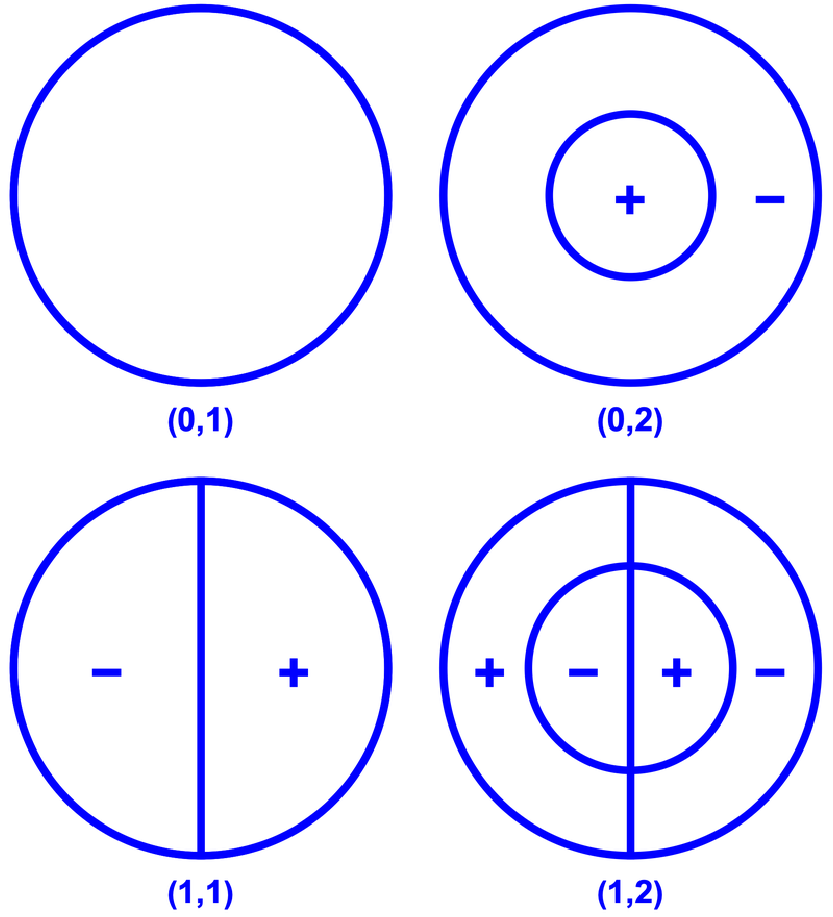
\includegraphics[width=0.5\textwidth]{normal modes.pdf}
	\caption{}
	\label{fig:normal modes memb}
\end{figure}
\section{Spherical Waves}
The spherical wave equation is governed by the Laplacian in spherical polar coordinates. The spherical wave equation is given by,
\begin{equation}
	\frac{1}{r^2}\pdv{r}\left(r^2\pdv{f}{r}\right) + \frac{1}{r^2\sin\theta}\pdv{\theta}\left(\sin\theta \pdv{f}{\theta}\right) + \frac{1}{r^2\sin^2\theta}\pdv[2]{f}{\phi} = \frac{1}{c^2} \pdv[2]{f}{t}.
\end{equation}
Let us for now consider the solution on the surface, $r = a$. Let us use a separation of variables, 
\begin{equation}
	F(\theta, \phi, t) = Y(\theta, \phi)T(t)
\end{equation}
We have,
\begin{equation}
	\frac{1}{Ya^2\sin\theta}\pdv{\theta}\left(\sin\theta \pdv{Y}{\theta}\right) + \frac{1}{Y a^2\sin^2\theta}\pdv[2]{Y}{\theta} = \frac{1}{c^2T}\dv[2]{T}{t} = -\frac{l(l+1)}{a^2}.
\end{equation}
Analysing the time equation,
\begin{equation}
	\dv[2]{T}{t} = - \frac{l(l+1)}{a^2c^2}T
\end{equation}
we have a trivial SHM solution,
\begin{equation}
	T = A\sin(\omega t) + B\cos(\omega t)
\end{equation}
where
\begin{equation}
	\omega^2 = \frac{c^2}{a^2}l(l+1).
\end{equation}
For the angular solution, we use separation of variables,
\begin{equation}
	Y = \Theta(\theta)\Phi(\phi)
\end{equation}
to obtain,
\begin{equation}
	\begin{split}
	\frac{1}{sin\theta}\dv{\theta}\left(\sin\theta\dv{\Theta}{\theta}\right) + \frac{1}{\sin^2\theta}\dv[2]{\Phi}{\phi} & = -l(l+1)\Theta\Phi \\
	\underbrace{\frac{\sin\theta}{\Theta}\dv{\theta}\left(\sin\theta\right) + l(l+1)\sin^2\theta}_{m^2} + \underbrace{\frac{1}{\Phi}\dv[2]{\Phi}{\phi}}_{-m^2} & = 0 
	\end{split}
\end{equation}
Let us consider a solution of constant $\phi$, and set $m=0$. Our equation is then purely in $\theta$,
\begin{equation}
	\frac{\sin\theta}{\Theta}\dv{\theta}\left(\sin\theta \dv{\Theta}{\theta}\right) + l(l+1)\sin^2\theta = 0.
\end{equation}
We can solve this by a substitution $x = \cos\theta$,
\begin{align}
	\dv{x}{\theta} =-\sin\theta && \implies && \dd{\theta} = - \frac{\dd{x}}{\sin\theta}
\end{align}
Our equation then becomes,
\begin{equation}
	-\frac{\cancelto{1}{\sin^2\theta}}{\Theta}\dv{x}\left(-\sin^2\theta \dv{\Theta}{x}\right) + l(l+1)\cancelto{1}{\sin^2\theta} = 0
\end{equation}
If we note that $\sin^2\theta = 1 - x^2$,
\begin{equation}
	\dv{x}\left((1-x^2)\dv{\Theta}{x}\right) + l(l+1)\Theta = 0
\end{equation}
which is Legendre's polynomials. Our solution is then,
\begin{equation}
	\Theta = P_{l}(x).
\end{equation}
The general solution, considering only $\theta$ and $t$ dependence is then,
\begin{equation}
	f(\theta, t) = \sum_{l=0}^{\infty}P_l(\cos\theta)\left(A_l\cos\omega t + B_l\sin\omega t\right)
\end{equation}
\subsection{$\phi$ Dependent Solution}
Let us now consider solutions where $m\neq 0$. Our angular equations become,
\begin{align}
	&\frac{1}{\Phi}\dv[2]{\Phi}{\phi} = -m^2 \label{eq:phi} \\
	&\frac{1}{\sin\theta} \dv{\theta}\left(\sin^2\theta \dv{\Theta}{\theta}\right) + \left[l(L +1)- \frac{m^2}{\sin^2\theta}\right]\Theta = 0  \label{eq:thetaa}
\end{align}
Eq. \eqref{eq:phi} is trivial,
\begin{equation}
	\Phi = A \sin m \phi + B \cos m \phi, \hspace{1em} m \in \mathbb{Z}^+.
\end{equation}
Eq. \eqref{eq:thetaa} can be solved if we consider,
\begin{align}
	x & = \cos\theta \\
	\dv{x}{\theta} & = -\sin \theta \therefore \dd{\theta} = \frac{\dd{x}}{\sin\theta}
\end{align}
we can rewrite eq. \eqref{eq:thetaa} as,
\begin{equation}
	\dv{x}\left(1 - x^2\dv{\Theta}{\theta}\right) + \left[l(l+1) - \frac{m^2}{1-x^2}\right]\Theta = 0.
\end{equation}
For $m=0$, we obtain Legendre polynomial solutions. However, for $m\neq0$, we obtain associated Legendre polynomials,
\begin{equation}
	\Theta = P_l^m(x), \hspace{1em} |m| \leq l.
\end{equation}
We then find the total angular solution is,
\begin{equation}
	Y(\theta, \phi) = P_l^m(\cos\theta)\left[A \sin m \phi + B \cos m \phi\right]
\end{equation}
\subsection{Waves Inside the Sphere ($r$ dependence)}
If we take into account $r$ dependence, we retain the angular solutions from before. Focusing on the radial and time solutions,
\begin{equation}
	\frac{1}{Rr^2}\dv{r}\left(r^2\dv{R}{r}\right) - \frac{l(l+1)}{r^2} = \frac{1}{c^2T}\dv[2]{T}{t} = -k^2. \label{eq:radial}
\end{equation}
We see the time solutions are SHM. Focussing on the radial equation,
\begin{equation}
	\dv{r}\left(r^2\dv{R}{r}\right) + \left[k^2r^2 - l(l+1)\right] = 0.
\end{equation}
Let us recall the boundary condition $R(a) = 0$, where $a$ is the surface of the sphere. Let $x=kr$ to rewrite eq. \eqref{eq:radial},
\begin{equation}
	\boxed{x^2\dv[2]{R}{x} + 2x\dv{R}{x} + \left[x^2 - l(l+1)\right]R = 0}
\end{equation}
which is the form of the \textit{spherical Bessel equation}. The solution to the spherical Bessel equation are the spherical Bessel functions,
\begin{equation}
	R = j_l(kr).
\end{equation}
\begin{aside}
	It can be shown that,
	\begin{equation}
		j_l(x) = \sqrt{\frac{\pi}{2x}}J_{l+\frac{1}{2}}(x).
	\end{equation}
\end{aside}
Applying the boundary condition,
\begin{equation}
	j_l(k_{lm}a) = 0.
\end{equation}
The final solution to the spherical wave equation is given by,
\begin{equation}
	f = \sum_{l,m,n}^{\infty}j_l(k_{ln}r)P_l^m(\cos\theta)\left[\sin(m \phi) + \cos( m \phi)\right]\left[A_{lmn}\cos(\omega_{lmn}t) + B_{lmn}\cos(\omega_{lmn}t)\right]
\end{equation}
\appendix
\chapter{Examples: Differential Equations}
\section{1D Wave Equation}
The 1 dimensional wave equation for a wavefunction $\phi$ is given by,
\begin{equation}
	\boxed{\pdv[2]{\phi}{x} = \frac{1}{c^2}\pdv[2]{\phi}{t}}. \label{eq:1dwave}
\end{equation}
\subsection{Euler/d'Alembert solution}
We can find a general solution to eq. \eqref{eq:1dwave} by using the substitution,
\begin{align}
	v & = x - ct \Leftarrow \text{ Backward component}\label{eq:backward}\\
	u & = x + ct \Leftarrow \text{ Forward component}\label{eq:forward}.
\end{align}
Computing the derivative with respect to $x$ by the chain rule,
\begin{equation}
	\pdv{\phi}{x} = \pdv{\phi}{v}\pdv{v}{x} + \pdv{\phi}{u}\pdv{\phi}{u} = \left(\pdv{v} + \pdv{u}\right)\phi
\end{equation}
from which the second derivative follows,
\begin{equation}
	\pdv[2]{\phi}{x} = \left(\pdv{u}+\pdv{v}\right)^2\phi. \label{eq:spacial}
\end{equation}
Similarly for the time component,
\begin{equation}
	\pdv[2]{\phi}{t} = c^2\left(\pdv{u}-\pdv{v}\right)^2\phi. \label{eq:time}
\end{equation}
Applying eqs. \eqref{eq:spacial} and \eqref{eq:time} to eq. \eqref{eq:1dwave}, we find,
\begin{equation}
	\begin{split}
		& \left(\pdv[2]{u} + \pdv[2]{v} + 2\pdv{u}\pdv{v}\right) = \frac{c^2}{c^2}\left(\pdv[2]{u} + \pdv[2]{v} - 2\pdv{u}\pdv{v}\right) \\
		\implies & \left(\pdv{u}\pdv{v}\right)\phi = 0 \implies \text{The solution is a sum of backward and forward components.}
	\end{split}
\end{equation}
Thus the general solution to eq. \eqref{eq:1dwave} is,
\begin{equation}
	\boxed{\phi = \phi(x + ct) - \phi(x-ct)}.
\end{equation}

\section{Laplace's Equation}
Laplace's equation is given by,
\begin{equation}
	\boxed{\grad^2\phi = 0}
\end{equation}
and can be readily solved using separation of variables.
\section{Diffusion Equation}
The diffusion equation is given by,
\begin{equation}
	\boxed{\grad^2T = \frac{1}{\alpha}\pdv{T}{t}}
\end{equation}
which reduces to Laplace's equation for a steady-state system. We will use it to analyse the temperature distribution on a circular plate.
\\\\
Given we have a circular plate, we wish to use the polar form of the Laplacian. We have,
\begin{equation}
	\frac{1}{r}\pdv{r}\left(r\pdv{T}{r}\right) + \frac{1}{r^2} \pdv[r]{T}{\theta} = \frac{1}{\alpha^2}\pdv{T}{t}.
\end{equation}
The circular plate has an insulating boundary, and has a cyclic boundary condition,
\begin{align}
	\eval{\pdv{T}{r}}_{r=a} = 0 \\
	T(r,\theta,t) = T(r, \theta + 2n\pi, t).
\end{align}
We then solve the diffusion equation by separation of variables, $T = R(r)\Theta(\theta)\tau(t)$,
\begin{equation}
	\frac{1}{Rr}\dv{r}\left(r\dv{R}{r}\right) + \frac{1}{\Theta r^2}\dv[2]{\Theta}{\theta} = \frac{1}{\alpha^2\tau}\dv{\tau}{t} = -k^2. \label{eq:fhdj}
\end{equation}
The \textit{time equation} is,
\begin{equation}
	\frac{\dd{\tau}}{\tau} = -k^2\alpha^2\dd{t}
\end{equation}
which has an exponential solution,
\begin{equation}
	\tau = Ae^{-k^2\alpha^2t}.
\end{equation}
Let us analyse the $\theta$ and $r$ dependence in eq. \eqref{eq:fhdj},
\begin{equation}
	\frac{r}{R}\left(r\dv{R}{r}\right) + k^2r^2 = - \frac{1}{\Theta}\dv[2]{\Theta}{\theta} = m^2
\end{equation} 
The cyclic equation is given by, 
\begin{equation}
	\dv{\Theta}{\theta} = -m^2\Theta
\end{equation}
which has a trigonometric solution,
\begin{equation}
	\Theta = A\cos(m\theta) + B\sin(m\theta)
\end{equation}
where we require $m \in \mathbb{N}^+$ to satisfy the cyclic boundary condition.
\\\\
The \textit{radial equation} is given by,
\begin{equation}
	\boxed{r^2\dv[2]{R}{r} + r\dv{r}{R} + (k^2r^2 - m^2)R = 0}
\end{equation}
which is Bessel's equation. The radial solution is then given by,
\begin{equation}
	R = J_m(kr)
\end{equation}
where $J_m(kr)$ is an $m^{\text{th}}$ order Bessel function.
\end{document}

\chapter{Misc. Notes}
\section{Plane Wave Nature}
We have that travelling waves in 3D are given by $e^{i(\vb{k}\cdot\vb{x})}$ and have a plane wave nature, such that,
\begin{equation}
	(\vb{k}\cdot\vb{x}-\omega t) = \phi
\end{equation}
where $\phi$ is constant. This corresponds to a plane wave with constant phase. So, we can write,
\begin{equation}
	\begin{split}
		& |\vb{k}||\vb{x}| - \omega = \phi \\
		\implies & |\vb{x}| = \frac{\omega t + \phi}{|\vb{k}|}
	\end{split}
\end{equation}
which is the equation of a sphere with radius $\frac{\omega t + \phi}{|\vb{k}|}$. Thus, a travelling wave in 3D represents spherical waves propagating outwards with velocity $\frac{\omega}{|\vb{k}|}$.
